\begin{titlepage}

\centering

\begin{tikzpicture}

\node[inner sep=0pt] (logo) at (0,0){
    
\includegraphics[width= .25\textwidth]{Figures/0. General/epfl-titlepage.png}};
    
\node[text width = 0.5\textwidth, right = of logo](title){\sffamily\huge\reporttitle};

\node[text width = 0.5\textwidth, yshift = 0.75cm, below = of title](subtitle){\sffamily\Large \reportsubtitle};

\gettikzxy{(subtitle.south)}{\sffamily\subtitlex}{\subtitley}
\gettikzxy{(title.north)}{\titlex}{\titley}
\draw[line width=1mm, Tue-red]($(logo.east)!0.5!(title.west)$) +(0,\subtitley) -- +(0,\titley);

\end{tikzpicture}
\vspace{1cm}

% table for group members -------------
\sffamily\groupnumber

\begin{table}[H]
    \centering
    \sffamily
    \large
    \begin{tabu} to 0.8\linewidth {cc}
        \textbf{Full Name} & \textbf{SCIPER}\\
        \hline
        \sffamily\reportauthors
        \end{tabu}
\end{table}


\vspace{0.3cm}

\sffamily \grouptutor

\vspace{0.3cm}

% table for dates ----------------
\begin{table}[H]
    \centering
    \sffamily
    \large
    \begin{tabu} to 0.8\linewidth {cc}
        \textbf{Lab Number} & \textbf{Date}\\
        \hline
        \sffamily\practicaldates
    \end{tabu}
\end{table}



\tikz[remember picture,overlay]\node[anchor=south,inner sep=0pt] at (current page.south) {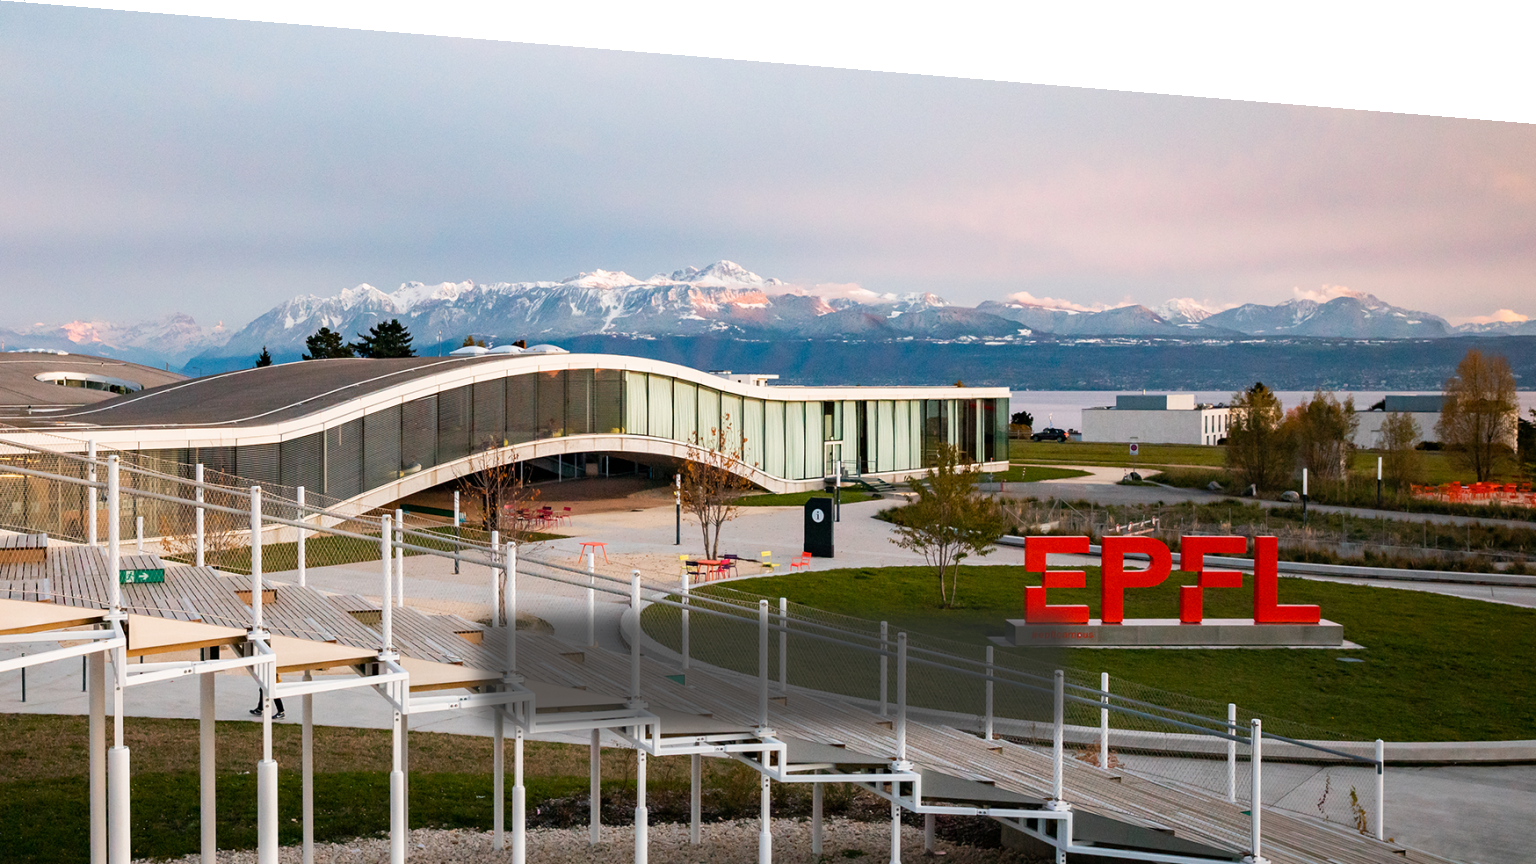
\includegraphics[width=\paperwidth]{Figures/0. General/epfl-landscape.png}};

\mbox{}
\vfill
\sffamily \Large \textcolor{white}{\placeanddate} \\



\end{titlepage}








